\mychapter{Sobre validação de código}\label{ch:apendiceD}

Este apêndice trata da validação de código Python em uma questão paramétrica antes de ser salvo no banco de dados. Esta é uma adaptação do Trabalho de Conclusão de Curso do Programa de Graduação em Ciência da Computação (área de concentração: Segurança da Informação), como parte dos requisitos necessários para a obtenção do título de Bacharel em Ciência da Computação do estudante Gabriel Tavares Frota de Azevedo. O trabalho foi desenvolvido no curso da Universidade Federal do ABC, no período de 2023-2024. 

Este apêndice começa apresentando a estrutura inicial de uma validação realizada na linguagem de programação Go, também conhecida como GoLang. Em seguida, apresenta a solução proposta pelo estudante Gabriel. Por fim, o apêndice apresenta um resumo do trabalho desenvolvido.


\section{Instalações e bibliotecas usadas}

\subsection{Instalação do Bandit}
O Bandit é uma ferramenta essencial para analisar vulnerabilidades em código Python. Para instalá-lo, utilize o seguinte comando:

\begin{verbatim}
    pip install bandit
\end{verbatim}

\subsection{Instalação do Go}
O Go é uma linguagem de programação desenvolvida pelo Google. Para instalá-lo, siga os seguintes passos:

\begin{enumerate}
    \item \textbf{Baixar o Go:} Baixe a versão 1.23.3 do Go (se necessário, utilize uma versão mais recente) em \href{https://go.dev/doc/install}{go.dev};
    \item \textbf{Extrair o Arquivo:} Extraia o arquivo baixado para o diretório /usr/local;
    \item \textbf{Atualizar o PATH:} Adicione o Go ao PATH do sistema para que os comandos Go estejam disponíveis no terminal;
    \item \textbf{Carregar as Alterações:} Atualize o PATH no terminal atual.
\end{enumerate}

\begin{verbatim}
    wget https://golang.org/dl/go1.23.3.linux-amd64.tar.gz
    sudo tar -C /usr/local -xzf go1.23.3.linux-amd64.tar.gz
    sudo sed -i '$ a export PATH=$PATH:/usr/local/go/bin' ~/.bashrc
    source ~/.bashrc
\end{verbatim}

\section{Criar um projeto simples para troca de mensagens}

Para criar um projeto Go simples que aplica requisições REST usando o método POST, seguir os passos abaixo. Este exemplo ilustrará como configurar um servidor básico que aceita dados em formato JSON via POST e retorna uma resposta.

\subsubsection{Estrutura do projeto}
Criar uma estrutura de diretório e arquivos como apresentado na Figura \ref{fig:estrutura-simple-rest-api}.

\begin{figure}[h!]%
    \centering
    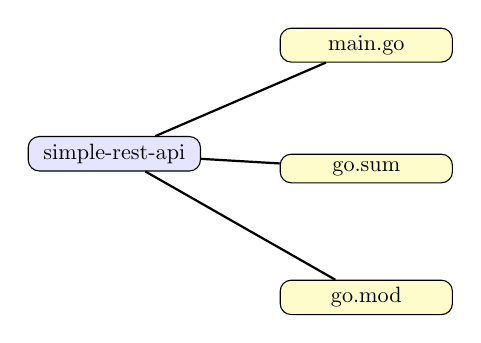
\begin{tikzpicture}[
        grow=right,
        edge from parent/.style={draw,thick},
        every node/.style={draw,rounded corners,anchor=north, align=center, text width=2.5cm}, % Ajuste de largura para 2.5cm
        level distance=4cm,
        sibling distance=2.5cm,
        scale=0.8,
        transform shape,
        folder/.style={rectangle, draw, fill=blue!10}, % Estilo para pastas com filhos
        file/.style={rectangle, draw, fill=yellow!20, text centered}, % Estilo para arquivos
        level 1/.style={sibling distance=2cm,level distance=4cm},
        level 2/.style={sibling distance=2.3cm,level distance=4cm},
        level 3/.style={sibling distance=0.9cm,level distance=4cm}
    ]
    \node[folder] {simple-rest-api}
        child {node[file] {go.mod}}
        child {node[file] {go.sum}}
        child {node[file] {main.go}};
\end{tikzpicture}
\caption{Diretório e arquivos de \texttt{simple-rest-api}.}
\label{fig:estrutura-simple-rest-api}
\end{figure}%


\subsubsection{Passo 1: Inicializar o projeto}

\begin{enumerate}
    \item Criar um novo diretório para o projeto:
    \begin{verbatim}
mkdir simple-rest-api
cd simple-rest-api
    \end{verbatim}

    \item Inicializar um novo módulo Go:
    \begin{verbatim}
go mod init simple-rest-api
    \end{verbatim}

    \item Adicionar a dependência do Gin:
    \begin{verbatim}
go get github.com/gin-gonic/gin
    \end{verbatim}
    Esse comando baixa e integra a biblioteca no ambiente de desenvolvimento, tornando possível utilizar as funcionalidades do Gin, como roteamento, manipulação de requisições HTTP e construção de APIs. 
\end{enumerate}

\subsubsection{Passo 2: Criar o arquivo \texttt{main.go}}

O Código \ref{lst:mainGo} (arquivo \texttt{main.go}) define uma API simples utilizando a biblioteca Gin. A estrutura \verb|Message| representa o formato JSON esperado para a requisição. O servidor disponibiliza uma rota POST em \verb|/message|. Quando a rota é acessada, o código decodifica o corpo da requisição para a estrutura \verb|Message|. Caso a validação do JSON falhe (campo \verb|text| ausente ou estrutura inválida), o servidor retorna um erro (\textit{HTTP Status Code 400 Bad Request}) com detalhes do erro. Se a validação for bem-sucedida, o servidor processa a mensagem e retorna uma resposta (\textit{HTTP Status Code 200 OK}) confirmando o recebimento do texto.

\begin{listing}[!ht]
    \begin{myboxCode}{corCodigo}{\textbf{Código Go: }}\vspace{3mm}
    \hrule
    \begin{minted}[xleftmargin=20pt,linenos=true]{GoLang}
package main
import (
    "net/http"
    "github.com/gin-gonic/gin"
)
type Message struct {
    Text string `json:"text" binding:"required"`
}
func main() {
    // Criar um roteador Gin
    r := gin.Default()
    // Definir a rota para o método POST
    r.POST("/message", func(c *gin.Context) {
        var msg Message
        // Bind JSON recebido à estrutura Message
        if err := c.ShouldBindJSON(&msg); err != nil {
            c.JSON(http.StatusBadRequest, gin.H{"error": err.Error()})
            return
        }
        // Retornar uma resposta com a mensagem recebida
        c.JSON(http.StatusOK, gin.H{"received": msg.Text})
    })
    // Executar o servidor na porta 8080
    r.Run(":8080")
}
\end{minted}
\end{myboxCode}
\caption{Exemplo de código Go para \texttt{main.go}.}
\label{lst:mainGo}
\end{listing}


\subsubsection{Passo 3: Executar o servidor}

Para executar o servidor, usar o seguinte comando:

\begin{verbatim}
        go run main.go
\end{verbatim}

Isso iniciará um servidor na porta 8080.

\subsubsection{Passo 4: Testar a API}

Testar a API usando \texttt{curl}. Aqui está um exemplo usando \texttt{curl}:

\begin{verbatim}
        curl -X POST http://localhost:8080/message \
        -H "Content-Type: application/json" \
        -d '{"text": "Hello, World!"}'
\end{verbatim}

\subsubsection{Resposta esperada}

Se tudo estiver configurado corretamente, a resposta deverá ser esta:

\begin{verbatim}
        {
            "received": "Hello, World!"
        }
\end{verbatim}

O diagrama apresentado na Figura \ref{fig:figGo01} ilustra a interação entre um cliente e um servidor de API durante uma requisição POST para o rota final \texttt{/message}. O cliente envia um JSON contendo a mensagem \texttt{"text": "Hello, World!"}. O servidor valida o formato JSON recebido. Se ocorrer um erro de validação, o servidor responde com um erro 400 (\textit{Bad Request}) informando que o campo \texttt{text} é obrigatório. Caso a validação seja bem-sucedida, o servidor processa a mensagem e retorna uma resposta 200 (\textit{OK}) com a mensagem recebida, confirmando o processamento. Veja a seguir uma captura de saída do servidor com a primeira requisição POST correta e duas requisições com erros:


\begin{myboxCode}{corCSV}{\textbf{Saída do servidor:}}\vspace{3mm}
    \hrule
    {\footnotesize
    \begin{verbatim}
    [GIN] 2024/11/15 - 10:09:12 | 200 |  2.730988ms |  ::1 | POST  "/message"
    [GIN] 2024/11/15 - 10:09:51 | 400 |   101.305µs |  ::1 | POST  "/message"
    [GIN] 2024/11/15 - 10:10:16 | 400 |    98.401µs |  ::1 | POST  "/message"
    \end{verbatim}
    }
    \end{myboxCode}
    

\begin{figure}[!ht]
    \centering
    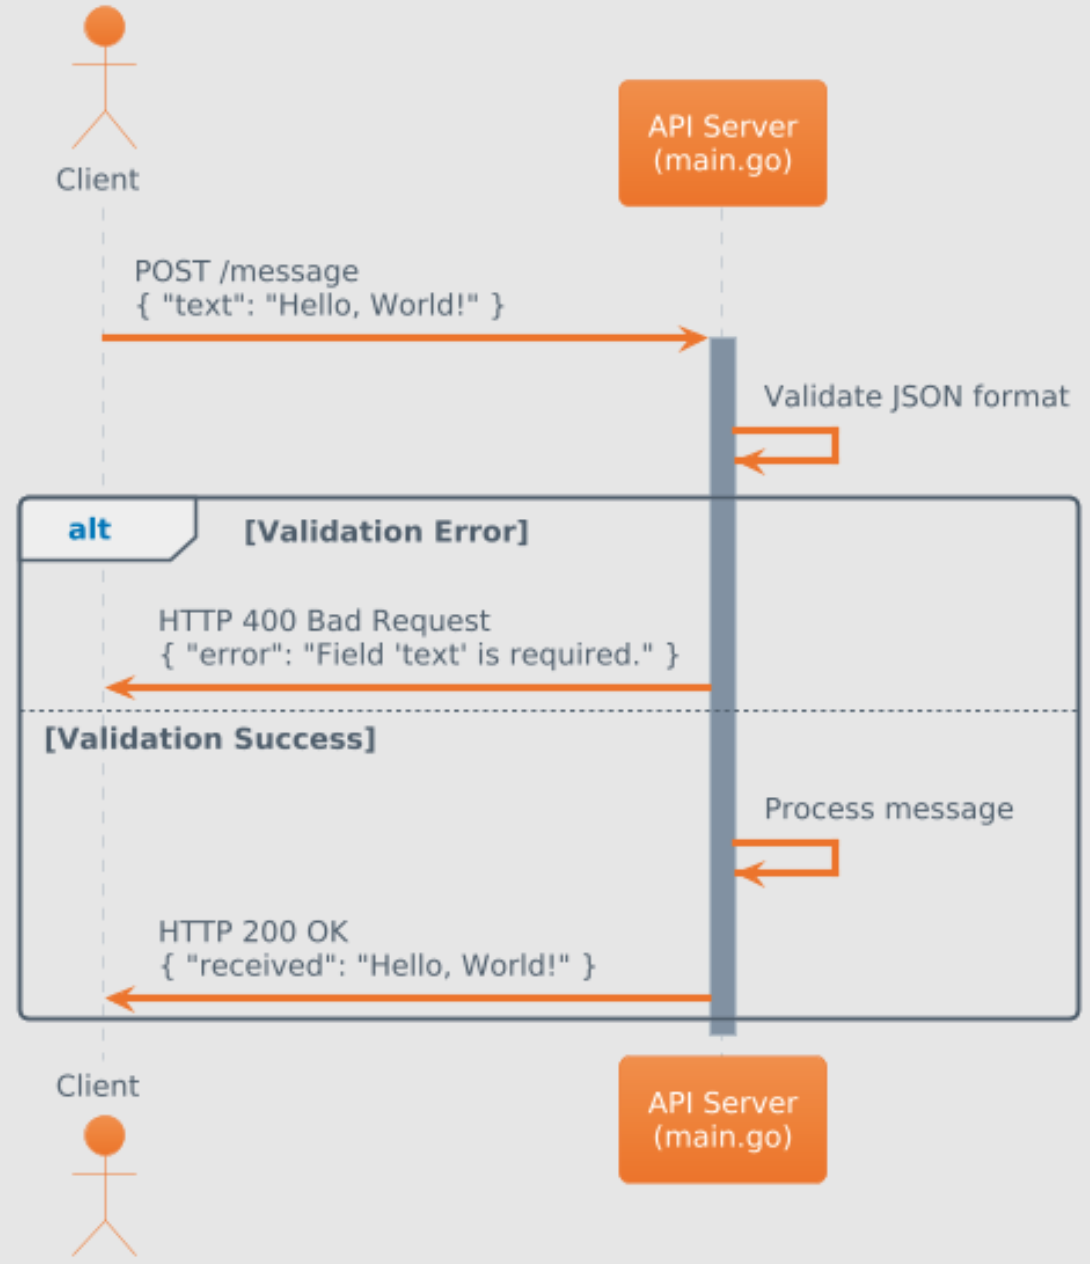
\includegraphics[width=0.7\textwidth]{ApeD_figGo01.png}
    \caption{Diagrama de sequência ilustrando a interação cliente-servidor para criar mensagens.}
    \label{fig:figGo01}
\end{figure}

Este exemplo é básico e pode ser expandido para incluir mais rotas, métodos HTTP, manipulação de erros, e integração com um banco de dados, como será apresentado na Seção \ref{sec:projeto-servidor-mctest-validator}. Antes, será apresentado como utilizar a bibliodeca \texttt{Bandit} para analisar segurança de código em Python.

\section{Exemplo simples de uso do \texttt{Bandit}}\label{sec:exemplo-bandit}

Nesta seção, será demonstrado um exemplo básico de utilização do \texttt{Bandit} para análise de segurança de código em Python. O \texttt{Bandit} é uma ferramenta que examina \textit{scripts} Python em busca de potenciais vulnerabilidades.

\subsection{Criação do arquivo \texttt{example.py}}

Primeiro, crie um arquivo chamado \texttt{example.py} com o conteúdo apresentado no Código \ref{lst:example.py}.

\begin{listing}[!ht]
    \begin{myboxCode}{corCodigo}{\textbf{Código Python: }}\vspace{3mm}
    \hrule
    \begin{minted}[xleftmargin=20pt,linenos=true]{Python}
import subprocess

def unsafe_method():
    subprocess.call('ls')  # Potencialmente inseguro
\end{minted}
\end{myboxCode}
\caption{Exemplo de código Python com potencial vulnerabilidade.}
\label{lst:example.py}
\end{listing}

O código acima contém um método \texttt{unsafe\_method} que utiliza o comando \texttt{subprocess.call} para executar um comando externo. Essa abordagem pode ser insegura, especialmente se as entradas do comando forem manipuladas por usuários externos.

\subsection{Instalação do \texttt{Bandit}}

Para instalar o \texttt{Bandit}, utilize o comando a seguir:

\begin{verbatim}
        pip install bandit
\end{verbatim}

\subsection{Análise do arquivo com o \texttt{Bandit}}

Após a instalação, execute o seguinte comando para realizar a análise de segurança no arquivo \texttt{example.py}:

\begin{verbatim}
        bandit -f json -r example.py
\end{verbatim}

Esse comando gera um relatório no formato JSON, identificando potenciais vulnerabilidades no código. O relatório apresenta detalhes, incluindo o trecho de código afetado, número da linha, links para documentação relevante, e recomendações para mitigar os riscos. O Código \ref{lst:Report-example.py} apresenta trecho desse JSON.
\begin{listing}[!ht]
    \begin{myboxCode}{corCodigo}{\textbf{Código JSON: }}\vspace{3mm}
    \hrule
    \begin{minted}[xleftmargin=20pt,linenos=true]{JSON}
{
  "errors": [],
  "generated_at": "2024-11-15T14:37:04Z",
  "metrics": {
    "./example.py": {
      "CONFIDENCE.HIGH": 3,
      "CONFIDENCE.LOW": 0,
      "CONFIDENCE.MEDIUM": 0,
      "CONFIDENCE.UNDEFINED": 0,
      "SEVERITY.HIGH": 0,
      "SEVERITY.LOW": 3,
      "SEVERITY.MEDIUM": 0,
      "SEVERITY.UNDEFINED": 0,
      "loc": 3,
      "nosec": 0,
      "skipped_tests": 0
    },
    ...
  },
  "results": [
    {
      "code": "1 import subprocess\n2 def unsafe_method():\n\
                3     subprocess.call('ls') # Potencialmente inseguro\n",
      ...
      "issue_confidence": "HIGH",
      "issue_cwe": {
        "id": 78,
        "link": "https://cwe.mitre.org/data/definitions/78.html"
      },
      "issue_severity": "LOW",
      "issue_text": "Consider possible security implications associated with \
                    the subprocess module.",
      "line_number": 1,
      "line_range": [
        1
      ],
      "test_id": "B404",
      "test_name": "blacklist"
    },
    ...
\end{minted}
\end{myboxCode}
\caption{Trechos do conteúdo JSON destacando potencial vulnerabilidade no Código \ref{lst:example.py}.}
\label{lst:Report-example.py}
\end{listing}



\subsection{Interpretação do relatório}

O relatório gerado pelo \texttt{Bandit} aplicado no arquivo \texttt{example.py}, conforme mostrado no Código \ref{lst:Report-example.py}, indica que o uso do método \texttt{subprocess.call} no método \texttt{unsafe\_method} pode introduzir vulnerabilidades no sistema. Isso ocorre porque comandos externos podem ser executados de forma incontrolada, especialmente quando as entradas não são validadas adequadamente.
%
A análise realizada pelo comando \texttt{bandit -f json -r example.py}, conforme o Código \ref{lst:example.py}, identificou três vulnerabilidades de baixa gravidade (\texttt{SEVERITY.LOW}), todas com alta confiança (\texttt{CONFIDENCE.HIGH}). Os alertas estão associados ao uso do módulo \texttt{subprocess} no método \texttt{unsafe\_method}, conforme descrito abaixo:

\begin{itemize}
    \item \textbf{Teste B404}: Destaca implicações de segurança relacionadas ao uso do módulo \texttt{subprocess}, conforme detalhado no link da CWE \href{https://cwe.mitre.org/data/definitions/78.html}{CWE-78}.
    \item \textbf{Teste B607}: Aponta riscos no uso de caminhos parciais para executáveis, o que pode causar falhas ou comportamentos inesperados.
    \item \textbf{Teste B603}: Identifica a possibilidade de execução de entradas não confiáveis ao utilizar \texttt{subprocess.call}, reforçando a necessidade de medidas preventivas.
\end{itemize}


\section{Projeto servidor \texttt{mctest-validator}}\label{sec:projeto-servidor-mctest-validator}

Este projeto foi desenvolvido pelo estudante Gabriel Tavares Frota de Azevedo e está disponível no GitHub: \href{https://github.com/leirbagseravat/mctest-validator-api}{\texttt{mctest-validator-api}}.


A sequência de instruções apresentada no Código \ref{lst:scriptMCTest} pode ser utilizada para instalar o projeto \texttt{mctest-validator-api} do GitHub do MCTest. A sequência instala a biblioteca \texttt{bandit}, baixa a linguagem de programação \texttt{Go} e baixa o projeto \texttt{mctest-validator-api} do GitHub, configura o Go e inicia o servidor.

\begin{listing}[!ht]
\begin{myboxCode}{corCodigo}{\textbf{Código Bash: }}\vspace{3mm}
\hrule
\begin{minted}[xleftmargin=20pt,linenos=true]{bash}
pip install bandit
# Instalar Go usando PPA - https://go.dev/wiki/Ubuntu
wget https://golang.org/dl/go1.23.3.linux-amd64.tar.gz
sudo tar -C /usr/local -xzf go1.23.3.linux-amd64.tar.gz
sudo sed -i '$ a export PATH=$PATH:/usr/local/go/bin' ~/.bashrc
source ~/.bashrc
git clone https://github.com/leirbagseravat/mctest-validator-api.git
cd mctest-validator-api
go mod tidy # Baixar e instalar as dependências
go run main.go > logfile.txt 2>&1 & # Executar a aplicação mctest-validator-api
\end{minted}
\end{myboxCode}
\caption{Trecho de instruções para a instalação do serviço \texttt{mctest-validator-api}.}
\label{lst:scriptMCTest}
\end{listing}

Esse conjunto de instruções apresentado no Código \ref{lst:scriptMCTest} foi incluído no \textit{script} de instalação \texttt{\_setup-all.sh}, disponível no GitHub do projeto do MCTest. Para mais detalhes, ver a Seção \ref{sec:instalacao} -- \nameref{sec:instalacao}.

\subsection{Ajuste no MCTest}\label{sec:contexto}

Os ajustes realizados no MCTest focaram nos serviços de criação e atualização de questões, envolvendo modificações nos arquivos \texttt{views.py} e \texttt{UtilsMCTest4.py}, localizados na pasta \texttt{topic} do projeto MCTest no GitHub \href{https://github.com/fzampirolli/mctest}{github.com/fzampirolli/mctest}. Durante o salvamento de uma questão, esses serviços validam os campos do formulário para assegurar que estão de acordo com os requisitos definidos. O objetivo dessas modificações é garantir que as questões estejam em conformidade com critérios de segurança e formatação.

Uma das alterações principais foi a criação do método \texttt{generateCode}, apresentada no Código \ref{lst:generateCode}, que foi incorporada ao arquivo \texttt{UtilsMCTest4.py}. Esse método utiliza os parâmetros \texttt{request}, \texttt{question} e \texttt{pk}, processando o texto da questão ao dividi-lo em linhas e eliminando espaços em branco desnecessários. Cada linha tratada é armazenada em uma lista, que é posteriormente concatenada na \textit{string} \texttt{mystr}, conforme ilustrado nas linhas 2 a 10 do código.

\begin{listing}[!ht]
    \begin{myboxCode}{corCodigo}{\textbf{Código Python: }}\vspace{3mm}
    \hrule
    \begin{minted}[xleftmargin=20pt,linenos=true]{python}
def generateCode(request, question, pk):
    AllLines = question.splitlines()
    for i in range(len(AllLines)):
        if AllLines[i].replace(" ", "") == "":
            AllLines[i] = AllLines[i][1:] + '\n'
        else:
            AllLines[i] = AllLines[i] + '\n'

    # Concatena as linhas em uma única string sem caracteres de retorno
    mystr = ''.join(AllLines).replace("\r", "")
    myDef = UtilsMC.get_code(mystr, 'def')

    if myDef is not None:
        import requests
        url = f'http://localhost:8080/mctest/validator/question/{pk}'
        files = {'file': '\n'.join(myDef)}
        r = requests.post(url, files=files)
        res = r.json()
        print(res)

        # Em caso de erro, formata e exibe a resposta JSON na página de erro
        if 'ERROR' == res['result']['status']:
            error_message = json.dumps(res, indent=4, sort_keys=True)
            return render(request, 'exam/exam_errors.html', 
                          {'error_json': error_message})
\end{minted}
\end{myboxCode}
\caption{Método que filtra código em Python da questão e valida em \texttt{mctest-validator}.}
\label{lst:generateCode}
\end{listing}


A \textit{string} resultante é passada para o método \texttt{get\_code} (linha 11), responsável por identificar definições de funções no texto da questão. Caso sejam detectadas definições de código Python delimitadas por ``\texttt{[[def:}'' e ``\texttt{]]}'', essas linhas são enviadas para validação por meio de uma requisição HTTP POST. A URL da API é construída dinamicamente utilizando o identificador \texttt{pk}. O Código \ref{lst:generateCode} apresenta os detalhes dessa operação.

A API de validação retorna um relatório no formato JSON, que é analisado para identificar possíveis erros. Caso algum erro seja detectado, uma mensagem detalhada é exibida ao usuário em uma página de erro. O método \texttt{generateCode}, ao identificar problemas, interrompe o fluxo de execução e retorna a validação. Caso contrário, o método \texttt{formset.save()} é acionado, e o usuário é redirecionado para a URL especificada. O arquivo \texttt{exam\_errors.html}, localizado na pasta \texttt{exam/template/exam}, foi modificado para incluir o tratamento do erro, caso existente, conforme apresentado no Código \ref{lst:erroHTML}, o qual processa o conteúdo JSON retornado pela API.

\begin{listing}[!ht]
    \begin{myboxCode}{corCodigo}{\textbf{Código HTML: }}\vspace{3mm}
    \hrule
    \begin{minted}[xleftmargin=20pt,linenos=true]{HTML}
...
<!-- Display JSON formatted error details -->

  <!-- Actions buttons -->
  <div class="text-right mt-4">
    <button onclick="window.history.back()" class="btn btn-outline-primary">
        
    </button>
    <hr>
  </div>
  <h4>
  
  </h4>
  <h4></h4>
  <pre>{{ error_json }}</pre>
...

\end{minted}
\end{myboxCode}
\caption{Trecho de código para tratar o conteúdo JSON retornado pelo \texttt{requests} do método \texttt{generateCode}.}
\label{lst:erroHTML}
\end{listing}


O método \texttt{generateCode} é utilizada nas \textit{views} \texttt{QuestionCreate} e \texttt{UpdateQuestion} no arquivo \texttt{views.py}, antes de as alterações serem salvas no banco de dados. O Código \ref{lst:updateQuestionView} exemplifica sua utilização em uma atualização de questão, com destaque para as linhas adicionadas.

\begin{listing}[!ht]
    \begin{myboxCode}{corCodigo}{\textbf{Código Python: }}\vspace{3mm}
    \hrule
    \begin{minted}[xleftmargin=20pt,linenos=true]{python}
...
#  Método criado por Gabriel Tavares Frota de Azevedo para o TCC do BCC/UFABC.
validation = UtilsMC.generateCode(request, question_inst.question_text, pk)
if validation is not None:
    return validation

question_inst.save()
...
\end{minted}
\end{myboxCode}
\caption{Trecho de código incluído na \textit{view} de atualização de questão para chamar o método \texttt{generateCode}}
\label{lst:updateQuestionView}
\end{listing}


O propósito do método \texttt{generateCode} é garantir a segurança e integridade das questões geradas, implementando um sistema eficiente de validação automatizada.

\subsection{Comunicação entre MCTest e \texttt{mctest-validator}}\label{sec:contexto}

A interação entre o MCTest e o \texttt{mctest-validator} utiliza a biblioteca \texttt{Requests}, uma ferramenta Python que facilita a manipulação de solicitações HTTP. Após a análise sintática da questão, o MCTest realiza uma requisição REST via método POST, enviando o código Python no corpo da solicitação para uma URL que inclui o identificador da questão.

O JSON retornado pelo \texttt{mctest-validator} contém um campo de \textit{status}, que determina se a questão passou na validação. Em caso de sucesso, a questão é salva no MCTest. Se falhar, o usuário é redirecionado para uma página de erro que detalha as razões da falha. Este processo assegura que apenas questões válidas sejam aceitas, mantendo a qualidade e integridade do sistema.


A Figura \ref{fig:pastas} ilustra a estrutura de arquivos e pastas do projeto \texttt{mctest-validator-api}. Esta estrutura demonstra a organização do código em diferentes diretórios, cada um responsável por uma parte específica da aplicação, como configuração, controladores, mapeadores e serviços. Essa divisão facilita a manutenção e evolução do projeto.

\begin{figure}[h!]%
\centering
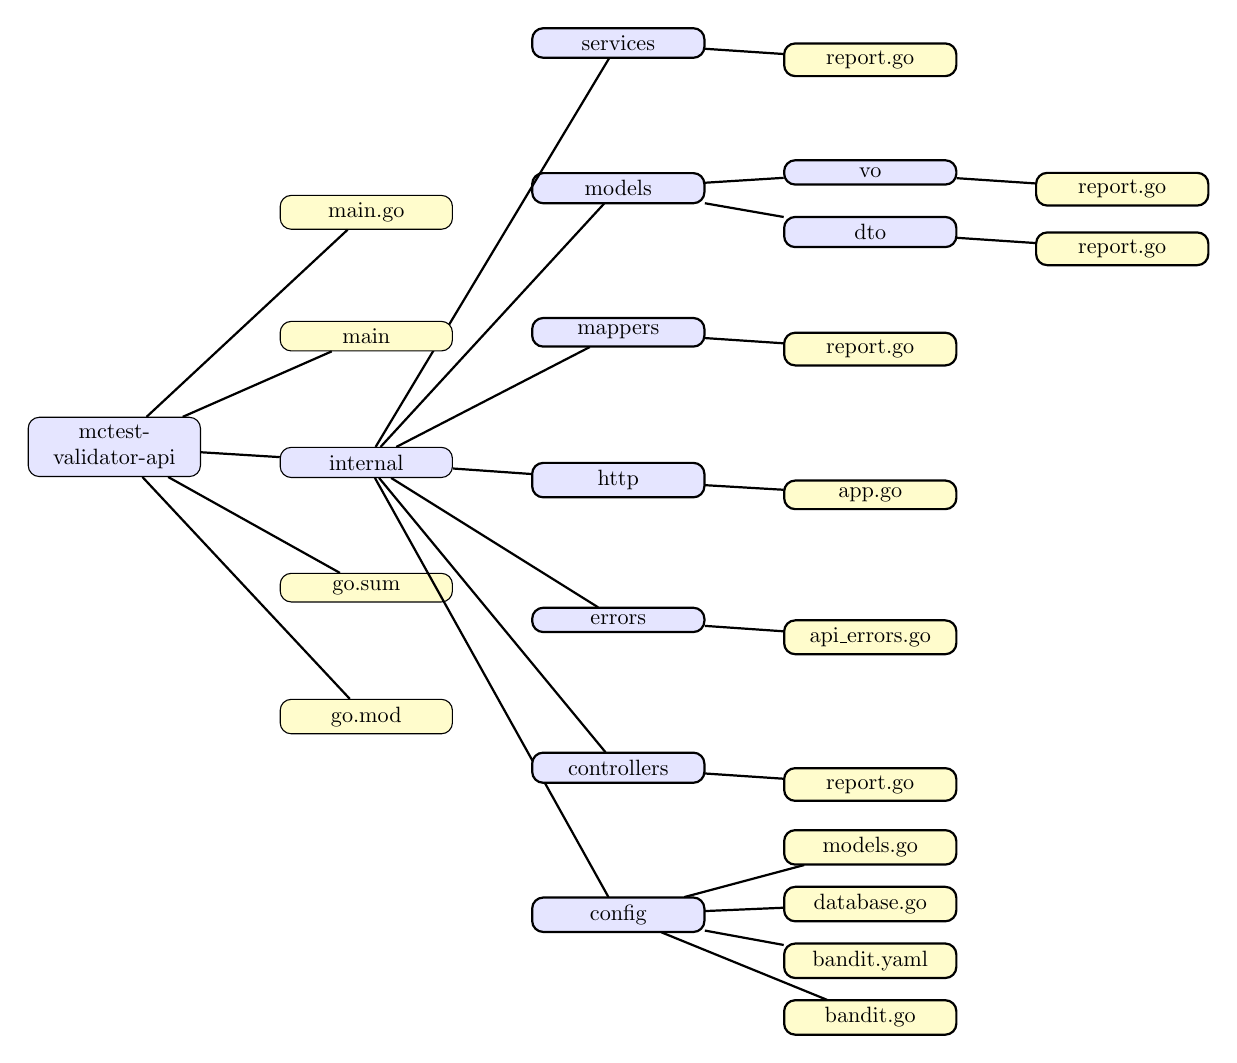
\begin{tikzpicture}[
    grow=right,
    edge from parent/.style={draw,thick},
    every node/.style={draw,rounded corners,anchor=north, align=center, text width=2.5cm}, % Ajuste de largura para 2cm
    level distance=4cm,
    sibling distance=2.5cm,
    scale=0.8,
    transform shape,
    folder/.style={rectangle, draw, fill=blue!10}, % Estilo para pastas com filhos
    file/.style={rectangle, draw, fill=yellow!20, text centered}, % Estilo para arquivos
    level 1/.style={sibling distance=2cm,level distance=4cm},
    level 2/.style={sibling distance=2.3cm,level distance=4cm},
    level 3/.style={sibling distance=0.9cm,level distance=4cm}
]
\node[folder] {mctest-validator-api}
    child {node[file] {go.mod}}
    child {node[file] {go.sum}}
    child {node[folder] {internal}
    child {node[folder] {config}
        child {node[file] {bandit.go}}
        child {node[file] {bandit.yaml}}
        child {node[file] {database.go}}
        child {node[file] {models.go}}
    }
    child {node[folder] {controllers}
        child {node[file] {report.go}}
    }
    child {node[folder] {errors}
        child {node[file] {api\_errors.go}}
    }
    child {node[folder] {http}
        child {node[file] {app.go}}
    }
    child {node[folder] {mappers}
        child {node[file] {report.go}}
    }
    child {node[folder] {models}
        child {node[folder] {dto}
        child {node[file] {report.go}}
        }
        child {node[folder] {vo}
        child {node[file] {report.go}}
        }
    }
    child {node[folder] {services}
        child {node[file] {report.go}}
    }
    }
    child {node[file] {main}}
    child {node[file] {main.go}};
\end{tikzpicture}
    \caption{Diretórios e arquivos de \texttt{mctest-validator}.}
    \label{fig:pastas}
\end{figure}%

O diagrama UML apresentado na Figura \ref{fig:plantuml} mostra a sequência de interações entre diferentes componentes da aplicação \texttt{mctest-validator-api}. Ele é dividido em três camadas:

\begin{itemize}
    \item \textbf{\textit{Application Layer}} (Camada de Aplicação): Inclui os participantes principais\\ \texttt{main.go}, \texttt{http/app.go} e \texttt{controllers/report.go}.
    \item \textbf{\textit{Domain Layer}} (Camada de Domínio): Contém a lógica de negócios e inclui\\
    \texttt{services/report.go}, \texttt{mappers/report.go}, \texttt{models/dto/report.go} e \texttt{models/vo/report.go}.
    \item \textbf{\textit{Infrastructure Layer}} (Camada de Infraestrutura): Responsável pelas operações de banco de dados com \texttt{config/database.go}.
\end{itemize}

O fluxo começa com \texttt{main.go} iniciando a aplicação, configurando o roteador e registrando rotas. Em seguida, a aplicação processa requisições HTTP, executa a lógica de negócios e interage com o banco de dados, retornando a resposta apropriada ao cliente.


\begin{figure}[h!]%
    \centering%
    \rotatebox{270}{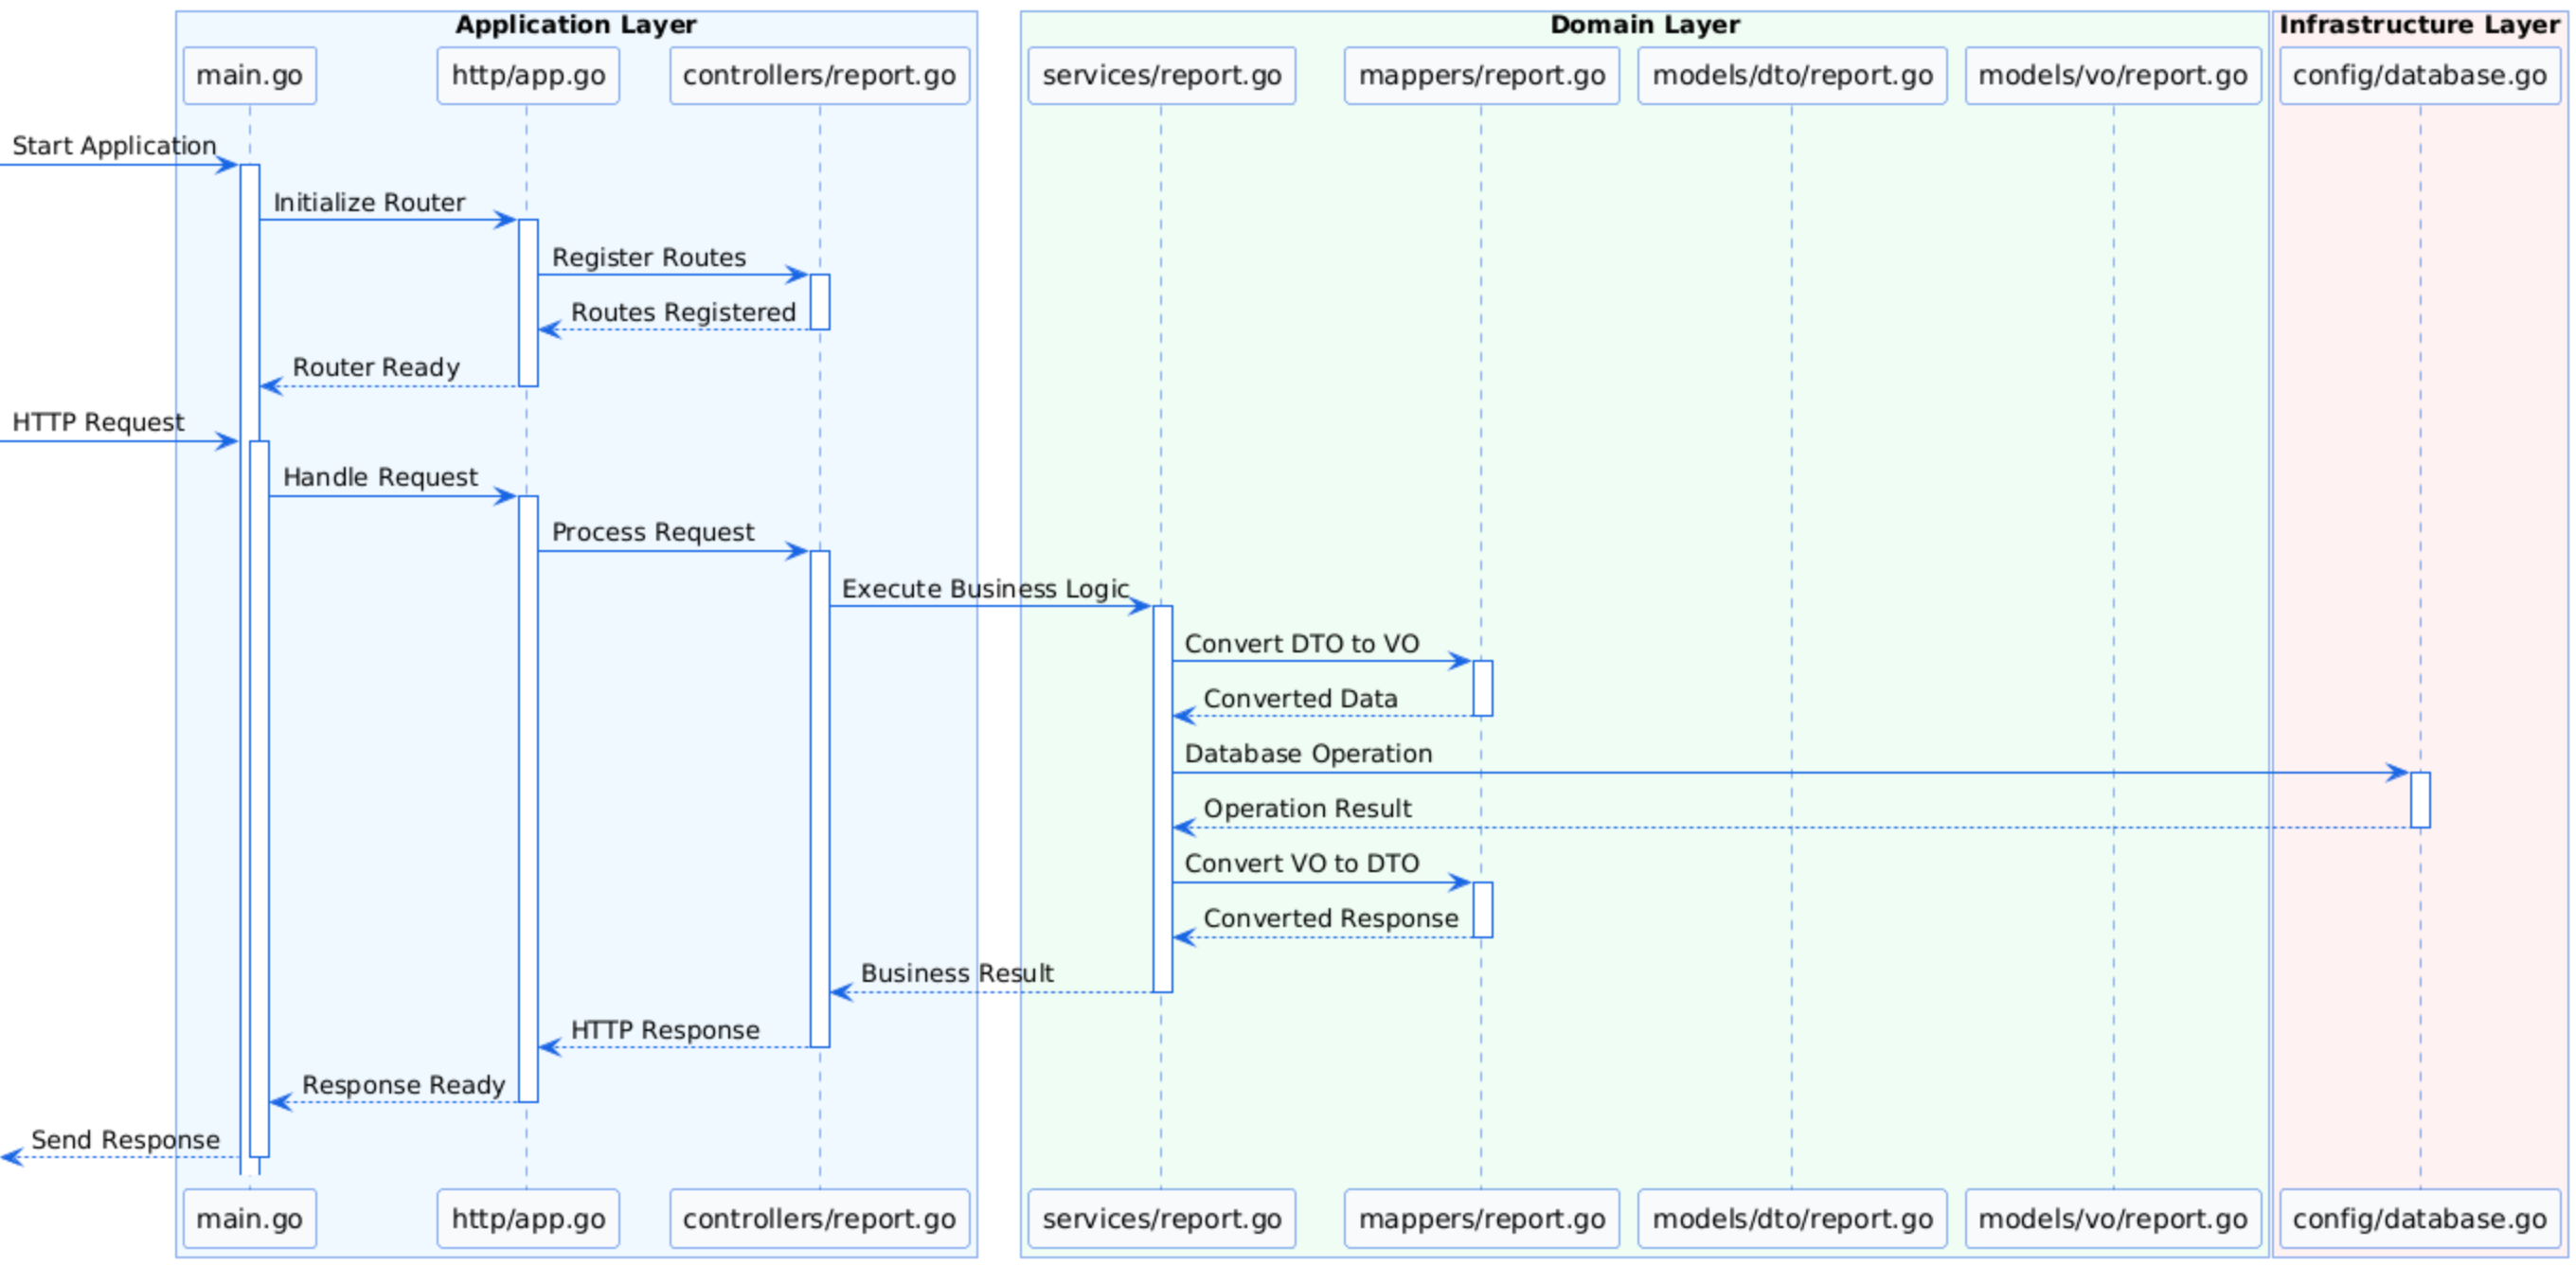
\includegraphics[width=0.96\textheight]{ApeD_plantuml.png}}
    \caption{Mensagens entre os diversos arquivos de \texttt{mctest-validator}.}
    \label{fig:plantuml}
\end{figure}%
% corrigir em https://www.plantuml.com/plantuml/uml/bLDDJzj04BtxLwp2EKr5FzH65OAGIY05WG1nwMcoEnjMEBlkx3X0g_xtJk9uxTWXQdDmh9ttvitRUJwD3CJbCi_Ya_C542pL7FJJWaBfpNd80wddHyVOgZ-2Dy_acD4h2tbiroB-BD5hLByp9Rypel1STJaw_lJv0ywhOys19e4CKhyuSnPdpkDRzHiWTjeLuFbV81qpH_QB1Qiti4busTVXJvRDmuiQd1L5xZIm2rxDu1Lf8EptzgkrMT48gC4Id7-t20C5KLt9-sxraRaOGL7K2Ecw2z31CuKyHueZmY8Grz3pLCdG6oL3RIUR1j7S6ShOZxjT8zBAQUoslAkEkmQAegz-jJdj88F1F8uCXmvuUd-z5xdg0X-kEruklIM8JANcah3nXFRO7lTkohh5o033728cxKdJSdYoMS5OtR4mLMk56MXsAs2iTfIjdqhW0XchI-_OGUv-eReD9ICbz6PVcJm4srh8MDtYmaL1LeIO2EsjDQzgM4jLy4H7andSnwq6_3OSjcWaD32lDIEDzoFPlhY_ln6GV8IH3pg-06zoR4CFsxsXe376Dg4_SjllIPsriVh-WheKwAICpg-RpCB2wTGYXJBRlWXvcxxnklqAYTS1KnmaFebM1xJwKyD6CR7Gg2amP0QxfBRKT38MM9KfTItLJbuaNzF9Rl-4alk8PSuj1O4VDFAmzY5s_jU821N1HpnefhEqTE5folwTzpEQKjGNRC3RaAJWrUYt4Yf1hhzCz7qtAQMdKYsN-Ly0


\section{Considerações finais}

Este apêndice apresentou uma solução para a validação de código Python em um contexto educacional, priorizando a segurança e a integridade dos dados. A integração do sistema de validação ao MCTest demonstrou a viabilidade de aplicar técnicas de análise de código estático em ambientes reais de ensino.

Como desdobramentos futuros, propõe-se: expandir o sistema para incorporar o uso de diferentes ferramentas de análise estática, com o objetivo de ampliar o espectro de vulnerabilidades detectáveis; aplicar técnicas de aprendizado de máquina para aumentar a precisão na detecção de vulnerabilidades e adaptar a análise ao contexto específico de cada questão; desenvolver mecanismos capazes de fornecer \textit{feedback} detalhado aos usuários em casos de erros; além de realizar testes de código estático, executar esse código e retornar as variáveis a serem utilizadas na questão, como os casos de teste utilizados na integração com o Moodle; e realizar testes de desempenho rigorosos, visando otimizar a eficiência e identificar possíveis gargalos no funcionamento do sistema.




